\documentclass{tufte-handout}

\usepackage{xcolor}

% set image attributes:
\usepackage{graphicx}
\graphicspath{ {images/} }

% set hyperlink attributes
\hypersetup{colorlinks}

% create environment for bottom paragraph:
\newenvironment{bottompar}{\par\vspace*{\fill}}{\clearpage}

\usepackage{enumerate}

% set table attributes
\usepackage{tabu}
\usepackage{booktabs}

% ============================================================

% define the title
\title{SOC 4015/5050: Lab 09 - Correlations By Hand}
\author{Christopher Prener, Ph.D.}
\date{Fall 2018}

% ============================================================

\begin{document}

% ============================================================

\maketitle % generates the title

% ============================================================

\vspace{5mm}
\section{Directions}
Please complete all steps below. Your your work ``by hand'' should be uploaded to your GitHub assignment repository by 4:15pm on Monday, November 5\textsuperscript{th}, 2017. 

\vspace{5mm}
\section{Correlation by Hand}
\vspace{3mm}
\noindent 
\begin{tabu} to 1\textwidth { X[r] X[r] X[l] X[r] X[r] X[r] }
 \multicolumn{6}{c}{2010 Missouri Congressional Election Results}\\
 \multicolumn{1}{c}{District} & \multicolumn{1}{c}{Population} & \multicolumn{1}{c}{Winner} & \multicolumn{1}{c}{Party} & \multicolumn{1}{c}{Incumbent} & \multicolumn{1}{c}{Turnout} \\
 \hline
 \hline
 1 & 587,000 & Clay & 1 & 1 & 184,779 \\
 2 & 706,600 & Akin & 0 & 1 & 265,632 \\
 3 & 625,300 & Carnahan & 1 & 1 & 203,085 \\
 4 & 680,000 & Hartzler & 0 & 0 & 225,056 \\
 5 & 634,000 & Cleaver & 1 & 1 & 191,423 \\
 6 & 700,000 & Graves & 0 & 1 & 221,912 \\
 7 & 722,000 & Long & 0 & 0 & 222,431 \\
 8 & 657,000 & Emerson & 0 & 1 & 195,999 \\
 9 & 683,000 & Luetkemeyer & 0 & 1 & 210,358 \\
 \hline
 \multicolumn{6}{l}{\textbf{\textit{Notes}}: Party value labels are 0 = Republican and 1 = Democrat; }\\ 
 \multicolumn{6}{l}{Incumbent value labels are 0 = No and 1 = Yes}\\
\end{tabu}
\vspace{3mm}

\begin{enumerate}
\item Calculate and fully interpret (including \textit{r}\textsuperscript{2}) the correlation between population and turnout in the table above. Does turnout appear to follow population size?
\item Calculate and fully interpret (including \textit{r}\textsuperscript{2}) the correlation between party and turnout in the table above. Are raw numbers of voters associated with turning out for races in which Democrats are the winners?
\item Calculate and fully interpret (including \textit{r}\textsuperscript{2}) the correlation between incumbency and turnout in the table above.  Are raw numbers of voters associated with incumbency?
\end{enumerate}

\vspace{5mm}
\section{Interpreting Scatterplots}
\begin{figure}[h]
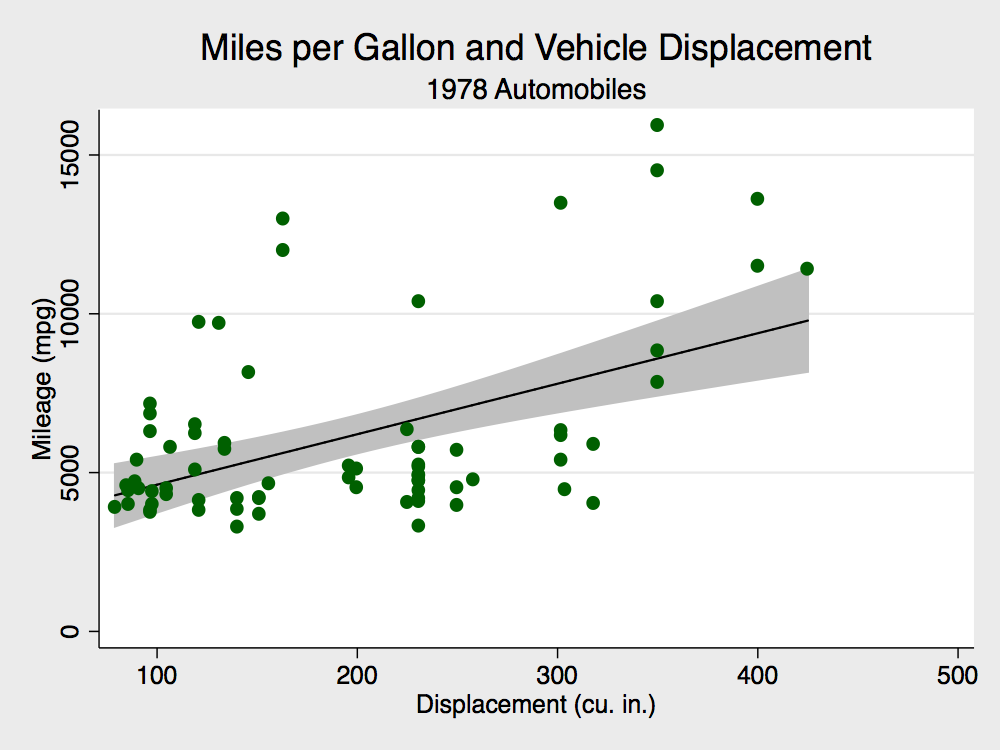
\includegraphics[scale=.46]{fig11.png}
\end{figure}

\vspace{3mm}
\begin{enumerate}
\setcounter{enumi}{3}
\item Interpret the scatterplot above. What do you think the direction and strength of the associated correlation coefficient are? Does the ``trend line'' appear to be a good model for the data?
\end{enumerate}

\newpage
\begin{figure}[h]
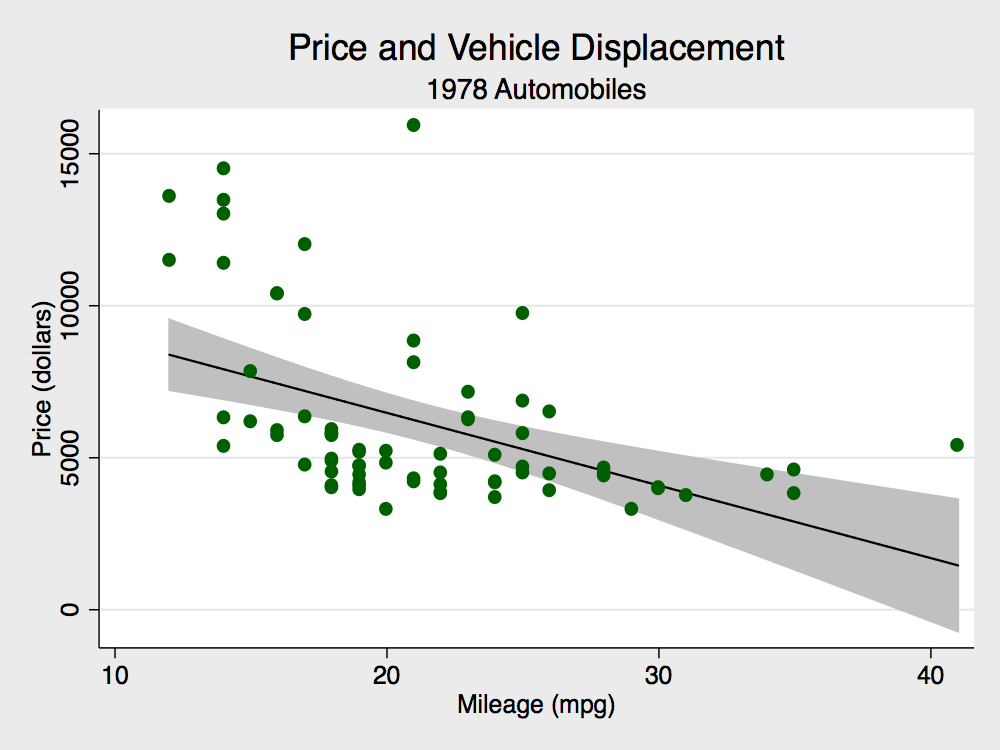
\includegraphics[scale=.46]{fig12.png}
\end{figure}

\vspace{3mm}
\begin{enumerate}
\setcounter{enumi}{4}
\item Interpret the scatterplot above. What do you think the direction and strength of the associated correlation coefficient are? Does the ``trend line'' appear to be a good model for the data?
\end{enumerate}

% ============================================================
\end{document}